\documentclass[a4paper]{article}
\usepackage{times}
\usepackage[utf8]{inputenc}
\usepackage{selinput}
\usepackage{upquote}
\usepackage[margin=2cm, rmargin=4cm, tmargin=3cm]{geometry}
\usepackage{tcolorbox}
\usepackage{xspace}
\usepackage[french]{babel}
\usepackage{url}
\usepackage{hyperref}
\usepackage{fontawesome5}
\usepackage{marginnote}
\usepackage{ulem}
\usepackage{tcolorbox}
\usepackage{graphicx}
%\usepackage[top=Bcm, bottom=Hcm, outer=Ccm, inner=Acm, heightrounded, marginparwidth=Ecm, marginparsep=Dcm]{geometry}


\newtcolorbox{Example}[1]{colback=white,left=20pt,colframe=slideblue,fonttitle=\bfseries,title=#1}
\newtcolorbox{Solutions}[1]{colback=white,left=20pt,colframe=green,fonttitle=\bfseries,title=#1}
\newtcolorbox{Conseils}[1]{colback=white,left=20pt,colframe=slideblue,fonttitle=\bfseries,title=#1}
\newtcolorbox{Warning}[1]{colback=white,left=20pt,colframe=warning,fonttitle=\bfseries,title=#1}

\setlength\parindent{0pt}

  %Exercice environment
  \newcounter{exercice}
  \newenvironment{Exercice}[1][]
  {
  \par
  \stepcounter{exercice}\textbf{Question \arabic{exercice}:} (\faClock \enskip \textit{#1})
  }
  {\bigskip}
  

% Title
\newcommand{\titre}{\begin{center}
  \section*{Algorithmes et Pensée Computationnelle}
\end{center}}
\newcommand{\cours}[1]
{\begin{center} 
  \textit{#1}\\
\end{center}
  }


\newcommand{\exemple}[1]{\newline~\textbf{Exemple :} #1}
%\newcommand{\attention}[1]{\newline\faExclamationTriangle~\textbf{Attention :} #1}

% Documentation url (escape \# in the TP document)
\newcommand{\documentation}[1]{\faBookOpen~Documentation : \href{#1}{#1}}

% Clef API
\newcommand{\apikey}[1]{\faKey~Clé API : \lstinline{#1}}
\newcommand{\apiendpoint}[1]{\faGlobe~Url de base de l'API \href{#1}{#1}}

%Listing Python style
\usepackage{color}
\definecolor{slideblue}{RGB}{33,131,189}
\definecolor{green}{RGB}{0,190,100}
\definecolor{blue}{RGB}{121,142,213}
\definecolor{grey}{RGB}{120,120,120}
\definecolor{warning}{RGB}{235,186,1}

\usepackage{listings}
\lstdefinelanguage{texte}{
    keywordstyle=\color{black},
    numbers=none,
    frame=none,
    literate=
           {é}{{\'e}}1
           {è}{{\`e}}1
           {ê}{{\^e}}1
           {à}{{\`a}}1
           {â}{{\^a}}1
           {ù}{{\`u}}1
           {ü}{{\"u}}1
           {î}{{\^i}}1
           {ï}{{\"i}}1
           {ë}{{\"e}}1
           {Ç}{{\,C}}1
           {ç}{{\,c}}1,
    columns=fullflexible,keepspaces,
	breaklines=true,
	breakatwhitespace=true,
}
\lstset{
    language=Python,
	basicstyle=\bfseries\footnotesize,
	breaklines=true,
	breakatwhitespace=true,
	commentstyle=\color{grey},
	stringstyle=\color{slideblue},
  keywordstyle=\color{slideblue},
	morekeywords={with, as, True, False, Float, join, None, main, argparse, self, sort, __eq__, __add__, __ne__, __radd__, __del__, __ge__, __gt__, split, os, endswith, is_file, scandir, @classmethod},
	deletekeywords={id},
	showspaces=false,
	showstringspaces=false,
	columns=fullflexible,keepspaces,
	literate=
           {é}{{\'e}}1
           {è}{{\`e}}1
           {ê}{{\^e}}1
           {à}{{\`a}}1
           {â}{{\^a}}1
           {ù}{{\`u}}1
           {ü}{{\"u}}1
           {î}{{\^i}}1
           {ï}{{\"i}}1
           {ë}{{\"e}}1
           {Ç}{{\,C}}1
           {ç}{{\,c}}1,
    numbers=left,
}

\newtcbox{\mybox}{nobeforeafter,colframe=white,colback=slideblue,boxrule=0.5pt,arc=1.5pt, boxsep=0pt,left=2pt,right=2pt,top=2pt,bottom=2pt,tcbox raise base}
\newcommand{\projet}{\mybox{\textcolor{white}{\small projet}}\xspace}
\newcommand{\optionnel}{\mybox{\textcolor{white}{\small Optionnel}}\xspace}
\newcommand{\advanced}{\mybox{\textcolor{white}{\small Pour aller plus loin}}\xspace}
\newcommand{\auto}{\mybox{\textcolor{white}{\small Auto-évaluation}}\xspace}


\usepackage{environ}
\newif\ifShowSolution
\NewEnviron{solution}{
  \ifShowSolution
	\begin{Solutions}{\faTerminal \enskip Solution}
		\BODY
	\end{Solutions}
  \fi}


  \usepackage{environ}
  \newif\ifShowConseil
  \NewEnviron{conseil}{
    \ifShowConseil
    \begin{Conseils}{\faLightbulb \quad Conseil}
      \BODY
    \end{Conseils}

    \fi}

    \usepackage{environ}
  \newif\ifShowWarning
  \NewEnviron{attention}{
    \ifShowWarning
    \begin{Warning}{\faExclamationTriangle \quad Attention}
      \BODY
    \end{Warning}

    \fi}
  

%\newcommand{\Conseil}[1]{\ifShowIndice\ \newline\faLightbulb[regular]~#1\fi}


\usepackage{array}
\usepackage{amsmath}
\usepackage{tabto}
\newcolumntype{C}[1]{>{\centering\let\newline\\\arraybackslash\hspace{0pt}}m{#1}}

\begin{document}

% Change the following values to true to show the solutions or/and the hints
\ShowSolutiontrue
\ShowConseiltrue
\titre
\cours{Probabilistic Algorithms}

Le but de cette séance est de comprendre les algorithmes probabilistes. Ceux-ci permettent de résoudre des problèmes complexes en relativement peu de temps. La contrepartie est que le résultat obtenu est généralement une solution approximative du problème initial. Néanmoins, ces algorithmes demeurent très utiles pour beaucoup d'applications.

\section{Monte-Carlo}
\begin{Exercice}[10 minutes]\textbf{Un jeu de hasard : Python}\\
Supposez que vous lanciez une pièce de monnaie \lstinline{l} fois et que vous voulez calculez la probabilité d'avoir un certain nombre de piles. Vous devez programmer un algorithme probabiliste, permettant de calculer cette probabilité. Pour ce faire, vous devez compléter la fonction \textit{proba(n,l,iter)} contenue dans le fichier \lstinline{Piece.py} (Dans le dossier \lstinline{Ressources}). La fonction \textit{Piece(l)} permet de créer une liste contenant des 0 et des 1 aléatoirement avec une probabilité $\frac{1}{2}$. Considérez un chiffre 1 comme une réussite (pile) et 0 comme un échec (face).
\\
\begin{conseil}
    Pour estimer empiriquement la probabilité d'un événement, comptez le nombre de fois que l'événement en question se produit en effectuant un nombre d'essai. Puis divisez le nombre d'occurrence de l'événement par le nombre total d'essai. Par exemple, si vous voulez estimer la probabilité d'obtenir un 2 avec un dé. Lancez le dé 1000 fois, comptez le nombre de fois que vous obtenez 2, et divisez le résultat par 1000.
\end{conseil}
\begin{solution}
    \lstinputlisting[language = python]{Piece_correction.py}
\end{solution}
\end{Exercice}

\begin{Exercice}[20 minutes]\textbf{Une approximation de $\pi$ : Python}\\
L'objectif de cet exercice est de programmer un algorithme probabiliste permettant d'approximer le chiffre $\pi$. Imaginez un plan sur lequel $0 < x < 1$ et $0 < y < 1$. Sur ce dernier, nous allons dessiner un quart de cercle centré en (0,0) et avec un rayon de 1. Par conséquent, un point dans cet espace se trouve à l'intérieur du cercle si $x^2 + y^2 < 1$. Vous trouverez ci-dessous une illustration de la situation:
\begin{center}
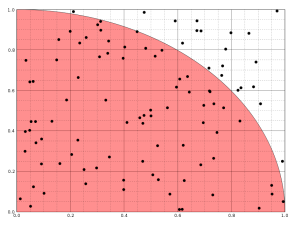
\includegraphics[]{Cercle.PNG}
\end{center}
La première étape de cet exercice consiste à créer une fonction permettant de déterminer si un point est à l'intérieur (zone rouge) ou à l'extérieur du cercle. Puis, générez 10000 points dans cet espace (x et y devrait appartenir à l'intervalle [0,1]). Pour ce faire, vous pouvez utliser la fonction \textit{random.random()} après avoir importé le module \textbf{random}. Vous pouvez obtenir l'approximation de $\pi$ à partir de la formule suivante : $\pi \approx [\frac{\text{Nombre de points dans le cercle}}{\text{Nombre total de points}}]\cdot 4$. Votre réponse devrait être assez proche du vrai chiffre $\pi$.\\
\begin{conseil}
    La fonction \lstinline{random.random()} génère aléatoirement un chiffre compris entre 0 et 1. Etant donné que vous devez simuler des points en 2 dimensions, vous devrez utiliser 2 fois cette fonction.
\end{conseil}
\begin{solution}
 \lstinputlisting[language = python]{Pi.py}
\end{solution}

\end{Exercice}
\newpage
\section{Fingerprinting}
\begin{Exercice}[20 minutes]\textbf{Fingerprinting: Une mission pour l'agente secrète Alice: Python}\\
    Dans cet exercice, vous prendrez le rôle de l'agente secrète Alice. Cette dernière enquêtait sur la disparition de son collègue,
    l'agent Bob, et se doutait que l'indice clé qui la mènerait à la vérité se trouvait dans la boîte mail de Bob. Alice arriva à trouver
    un bout de papier avec écrit dessus : ``\textit{Mon mot de passe est l'empreinte de ceciestmonmotdepasse}''. Aidez Alice à trouver l'empreinte du mot de passe! \\

    Pour cela, vous devez compléter deux fonctions :
    \begin{enumerate}
        \item \lstinline{is_a_prime_number(num)} qui vérifie que \lstinline{num} est un nombre premier ou pas. Un nombre premier est un entier naturel 
        qui admet exactement deux diviseurs distincts entiers et positifs. Ces deux diviseurs sont 1 et le nombre considéré, 
        puisque tout nombre a pour diviseurs 1 et lui-même, les nombres premiers étant ceux qui n’en possèdent aucun autre.
        
        \item \lstinline{fingerprinting(p, message)} qui implémente l'algorithme de fingerprinting suivant :
              \begin{enumerate}
                  \item Si \lstinline{p} est un nombre premier, calculez la valeur de hachage de la chaîne à l'aide de la fonction \lstinline{hash(...)}, puis calculez le modulo du résultat du hachage.
                  \item Sinon, imprimez un message qui dit que le nombre n'est pas un nombre premier.    
              \end{enumerate}
    \end{enumerate}

    Si vous réussissez à implémenter les deux fonctions correctement, le code vous imprimera : \lstinline{Connection réussie? True}.

    À vos ordis, détectives!

    \lstinputlisting[language = python]{fingerprinting.py}

    \begin{solution}
        \lstinputlisting[language = python]{fingerprinting_solution.py}
    \end{solution}
\end{Exercice}
\newpage
\section{Las Vegas}
\begin{Exercice}[10 minutes] \textbf{Quicksort - Algorithme de Las Vegas: Python}\\
    Un algorithme de Las Vegas est un algorithme probabiliste qui a la particularité de toujours trouver le résultat correct lorsqu'il existe. Son inconvénient est que sa compléxité temporelle ne peut être garantie à l'avance car elle dépend des données passées en paramètres.

    Dans cet exercice, vous allez implémenter un algorithme de tri rapide (quicksort) sur une liste d'éléments.
\\\\
    L'algorithme de tri rapide applique un paradigme \textit{divide-and-conquer} afin de trier un ensemble de nombres~\lstinline{A}. Il fonctionne en trois étapes: 
    \begin{enumerate}
        \item il choisit d'abord un élément pivot, \lstinline{A[q]}, en utilisant un générateur de nombres aléatoires (d'où sa nature d'algorithme dit probabiliste) ;
        \item puis il réorganise le tableau en deux sous-tableaux $A[p...q-1]$ et $A[q+1...r]$, où les éléments des premier et deuxième tableaux sont respectivement plus petits et plus grands que $A[q]$.
        \item L'algorithme applique ensuite récursivement les étapes de tri rapide ci-dessus sur les deux tableaux indépendants, produisant ainsi un tableau entièrement trié.
    \end{enumerate}
    \begin{figure}[h]
        \centering
        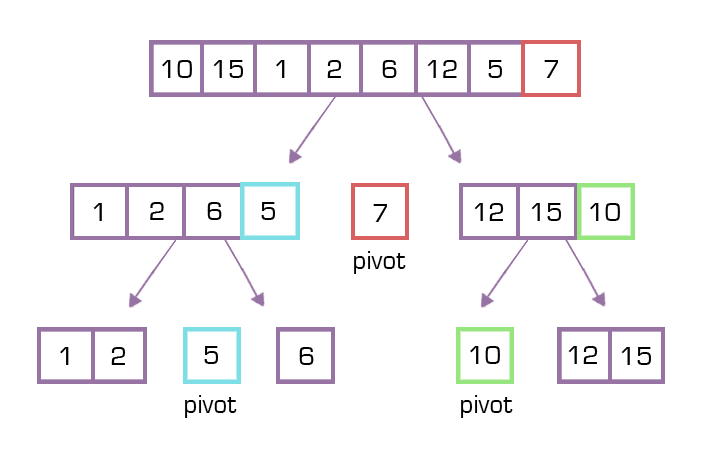
\includegraphics[width=\linewidth]{quicksort.png}
        \caption{Illustration de l'algorithme de tri rapide}
    \end{figure}

    Complétez le code suivant:
    \lstinputlisting[language = python]{quicksort.py}


    \begin{conseil}
        Pour le choix de votre élément pivot, pensez à utiliser la méthode \lstinline{randint()} de la librairie \lstinline{random}.
    \end{conseil}


    \begin{solution}
        \lstinputlisting[language = python]{quicksort_solution.py}
    \end{solution}
     


\end{Exercice}
\newpage
\section{Chaînes de Markov}

\begin{Exercice}[15 minutes]\textbf{Un exemple simple de la chaîne de Markov}

Les slides nous ont donné un exemple de la chaîne de Markov. Celui-ci comprend une matrice de transition et un calcul des probabilités de  3 états $x=(1,2,3)$ ($x$ est un vecteur ayant 3 éléments) à $t+3$  i.e $x^{(t+3)}$. Avant de continuer, assurez-vous que vous comprenez la formule de la \href{https://fr.wikipedia.org/wiki/Probabilit\%C3\%A9_conditionnelle}{\color{cyan} probabilité conditionnelle} dans les slides, et les opérations basiques de matrices et vecteurs qui y sont présentées (\href{https://fr.wikiversity.org/wiki/Initiation_aux_matrices/Puissance_d\%27une_matrice}{\color{cyan} puissance} et \href{https://fr.wikipedia.org/wiki/Produit_scalaire}{\color{cyan} produit scalaire}).\\

On va formaliser le concept de la chaîne de Markov avec les notations suivantes.\\
\begin{enumerate}
    \item Un processus ou une séquence $X_0, X_1, X_2, ..., X_n$ ($0,1,2,...,n$ signifiant de différents moments) est une chaîne de Markov si
    \begin{align} 
    P\Big(X_{n+1}=j | X_0=i_0, X_1=i_1, ... , X_{n-1}=i_{n-1},X_n=i\Big) = P\left(X_{n+1}=j | X_n=i\right).
    \end{align}
    En d'autres termes, toute information utile pour la prédiction du futur de la valeur $X$ d'une chaîne de Markov est uniquement dans l'état présent.
     
\item  Le nombre $P\left(X_{n+1}=j | X_n=i\right)$ est appelé \textit{probabilité de transition} de l'état $i$ à l'état $j$ (en un pas), et on écrit:
\begin{align}
p_{ij} = P\left(X_{n+1}=j | X_n=i\right)
\end{align}

La matrice $\mathbf{P}$ dont l'élément à l'indice $(i,j)$ (ligne $i$, colonne $j$) est $p_{ij}$ est appelée \textit{matrice de transition}. Si on a $N$ états, $P$ est de dimension $N \times N$ ($N$ lignes et $N$ colonnes). Si les chaînes sont homogènes, $\mathbf{P}$ \textbf{a deux propriétés importantes}: i, $p_{ij} \geq 0$ et ii, $\sum_i p_{ij} = 1$ (i.e chaque élément de la matrice est supérieur ou égal à 0, et la somme des probabilités à chaque ligne est toujours égale à 1).

\item Soit $\mu_n = (\mu_n(1), ..., \mu_n(N))$ un vecteur-ligne des probabilités, avec $\mu_n(i) = P(X_n=i)$. Par exemple, si on a 3 états et $\mu_2 = (0.5, 0.2, 0.3)$, on peut dire qu'à temps 2, la probabilité est 0.5 qu'on soit à l'état 1, 0.2 qu'on soit à l'état 2, et 0.3 qu'on soit à 3. \textbf{La variable $x^{(t+3)}$ des slides serait $\mu_3$ avec ces notations}!

$\mu_n$ est aussi appelée probabilités marginales, qui indiquent les probabilités des états à temps $n$, et elles sont calculées comme suit (vérifiez que cette formule s'accorde avec le calcul de $x^{(t+3)}$ des slides) :
\[ 
\mu_n = \mu_0 \mathbf{P}^n
\]
$\mu_0$ est donc appelée \textit{la loi initiale} (la loi de $X_0$); dans les slides, $\mu_0 = (0,\; 1, \; 0)$. En général, on a qu'à connaître $\mu_0$ et $\mathbf{P}$ pour simuler une chaîne de Markov. Cette information sera utile pour l'exercice 7 et 8. \\ 
\end{enumerate}

Et on a ci-dessous un résumé de la terminologie:

\begin{enumerate}
    \item $\mathbf{P}(i,j)$ : élément à ligne $i$ et colonne $j$ de la matrice $\mathbf{P}$.
    \item Matrice de transition $\mathbf{P}$ a $\mathbf{P}(i,j) = P(X_{n+1}=j|X_n=i)=p_{ij}$.
    \item $\mathbf{P}_n = \mathbf{P}^n$.
    \item Probabilité marginale : $\mu_n(i) = P(X_n = i)$.
    \item $\mu_n = \mu_0 \mathbf{P}^n$
\end{enumerate}

Etant donné que $X_0, X_1, ...$ est une chaîne de Markov avec 3 états $\{0, 1, 2\}$ et la matrice de transition:

\[ 
\mathbf{P} =
\begin{bmatrix}
0.1 & 0.2 & 0.7 \\
0.9 & 0.1 & 0.0 \\
0.1 & 0.8 & 0.1
\end{bmatrix}
\]
Supposons que $\mu_0 = (0.3, \; 0.4, \; 0.3)$. Trouvez $P(X_0 = 0, X_1=1, X_2=2)$ et $P(X_0=0, X_1=1, X_2=1)$.

\begin{conseil}
    Cet exercice vous demande de trouver deux probabilités \textbf{jointes}. Peut-être vous rappelez-vous qu'en général, 
    \[ 
    P(X=x, Y=y) = P(X=x)P(Y=y|X=x).
    \]
    Pouvez-vous le reformuler avec 3 variables ? En plus, notez bien que $X_0, X_1, ...$ est une chaîne de Markov i.e $P\Big(X_{n+1}=j | X_0=i_0, X_1=i_1, ... , X_{n-1}=i_{n-1},X_n=i\Big) = P\left(X_{n+1}=j | X_n=i\right)$. 
\end{conseil}

\begin{solution}
\begin{align*}
    1. \; &P(X_0=0,X_1=1, X_2=2) \\ 
    &= P(X_2=2|X_1=1,X_0=0)P(X_1=1|X_0=0)P(X_0 =0) \text{ (Bayes, règle de chaîne)}\\
    &= P(X_2=2|X_1=1)P(X_1=1|X_0=0)P(X_0=0) \text{ (définition de la chaîne de Markov)}\\ 
    &=p_{12} \times p_{01} = 0.3 \times 0.2 \times 0.0 = 0.0\\
    \\
    2. \; & P(X_0=0,X_1=1, X_2=1)=P(X_0 =0)\times p_{01} \times p_{11}\\
    &= 0.3 \times 0.2\times 0.1 = 0.006
\end{align*}
\end{solution}

\end{Exercice}

\begin{Exercice}[10 minutes]\textbf{Probabilités marginales: Python}

En utilisant la loi initiale $\mu_0$ et la matrice \textbf{P} de la question précédente, trouvez $\mu_1$, $\mu_2$.

\begin{conseil}
    Relisez et familiarisez-vous avec les notations et la terminologie ci-dessus! Si les slides s'avèrent plus utiles, considérez $\mu_1 = x^{(t+1)}, \mu_2 = x^{(t+2)}$.
\end{conseil}

On peut aussi essayer de les trouver en écrivant un programme Python! Nous vous fournissons une fonction qui calcule le produit scalaire entre un vecteur et une matrice. Essayez d'écrire une fonction pour trouver la puissance d'une matrice (en utilisant la fonction de produit scalaire) et puis une autre fonction pour les probabilités marginales.

\lstinputlisting[language=python]{ProbMarginales_temp.py}

\begin{conseil}
    Souvenez-vous que $\mathbf{P}^2$ est le produit scalaire entre $\mathbf{P}$ et $\mathbf{P}$! Chaque ligne de  $\mathbf{P}^2$ sera donc le produit scalaire entre une ligne de $\mathbf{P}$ et $\mathbf{P}$.
\end{conseil}
\begin{solution}
\begin{align}
\mu_1 &= \mu_0 \mathbf{P}^1 =
\left(\begin{matrix}
0.42 & 0.34 & 0.24
\end{matrix}\right)\\
\mu_2 &= \mu_0 \mathbf{P}^2 =
\left(\begin{matrix}
0.37 & 0.31 & 0.32
\end{matrix}\right) 
\end{align}

\lstinputlisting[language=python]{ProbMarginales.py}

\end{solution}

\end{Exercice}

\begin{Exercice}[20 minutes]\textbf{Simuler une chaîne de Markov: Python}\\
Pour cet exercice, vous n'avez pas à utiliser les calculs des exercices précédents.\\

Comme mentionné plus haut, la simulation d'une chaîne de Markov ($X_0, X_1, ...$) exige seulement deux éléments: la loi initiale $\mu_0$ et la matrice de transition $\mathbf{P}$. Spécifiquement, l'algorithme est:

\begin{enumerate}
    \item Supposer que les probabilités initiales (les probabilités des états potentiels de $X_0$) sont dans le vecteur $\mu_0$. Trouver $X_0$.
    \item Le résultat de l'étape 1 est donc $X_0 = i$, l'état de $X$ à temps 0; obtenir $X_1$ selon les probabilités à la $i$th ligne de $\mathbf{P}$ où $P(X_1=j|X_0=i)=p_{ij}$. Trouver $X_1$.
    \item Le résultat de l'étape 2 est $X_1 = j$, l'état de $X$ à temps 1; obtenir $X_2 \sim \mathbf{P}$ où $P(X_2=k|X_1=j)=p_{jk}$.
    \item Répéter jusqu'à la fin (le nombre d'iterations est arbitraire).
\end{enumerate}

Écrivez une fonction simple afin d'implémenter l'algorithme ci-dessus. Nommez-la \textbf{sim\_markov()}, celle-ci prend comme paramètres \textbf{P}, \textbf{mu\_0} et \textbf{n\_iters}. Essayez avec des valeurs différentes de \textbf{P}, \textbf{mu\_0} et \textbf{n\_iters}.
\lstinputlisting[language=python]{SimMarkov_temp.py}


\begin{conseil}
    Pensez à utiliser la méthode \textbf{random.choices()}. Elle vous permet de sélectionner de façon (pseudo-)aléatoire des éléments d'une liste. N'hésitez pas à vous référer à la documentation officielle pour plus de détails.
\end{conseil}
\begin{solution}
\lstinputlisting[language = python]{SimMarkov.py}
\end{solution}
\end{Exercice}

\begin{Exercice}[20 minutes]\textbf{Coder une chaîne de Markov avec un dictionnaire Python}

Cette fois-ci, vous allez utiliser un dictionnaire au lieu de vecteurs et matrices!

Supposez qu'il y'ait trois choix d'états avec les transitions dans l'image ci-dessous. Supposez également que la loi initiale des états est (0.3, 0.2, 0.5) pour \textbf{Sunny, Snowy, et Rainy} respectivement. Simulez une chaîne de Markov en utilisant un dictionnaire imbriqué, écrit comme suit
\lstinputlisting[language=python]{WeatherMarkovDict.py}
\begin{center}
        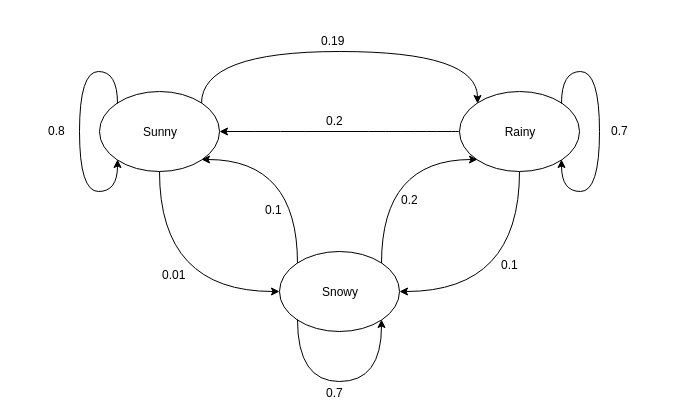
\includegraphics[width=\linewidth]{Etats_markov.png}
\end{center}
    
Complétez le programme ci-dessous.
\lstinputlisting[language=python]{WeatherMarkov_temp.py}

\begin{conseil}
    De nouveau, pensez à utiliser la méthode \textbf{random.choices()}.
\end{conseil}
\begin{solution}
    \lstinputlisting[language=python]{WeatherMarkov.py}
\end{solution}
\end{Exercice}

\newpage
\section{Treap}
\begin{Exercice}[20 minutes]\textbf{Insertion dans une Treap: Python} \optionnel\\
    Une Treap est un arbre binaire où chaque sommet $v$ a 2 valeurs, une clé \lstinline{v.key} et une priorité \lstinline{v.priority}. Une treap est une
    combinaison d'un arbre de recherche binaire et d'une heap. Ainsi, la treap a la même structure qu'un arbre de recherche binaire dont les nœuds sont
    insérés par ordre de priorité. \\

    Dans cet exercice, vous allez implémenter une fonction pour insérer un nœud dans une treap. Vous avez le squelette de code suivant à remplir.
    \lstinputlisting[language = python]{treap.py}

    \begin{conseil}
        La fonction \lstinline{insertNode} est récursive. Inspirez-vous de l'insertion dans un arbre de recherche binaire, mais 
        n'oubliez pas de vérifier que la propriété de la heap est satisfaite après avoir inséré. \\\\
        La propriété de la heap à satisfaire est que la priorité de la racine doit toujours être plus grande que celle de ses nœuds enfants.
        \lstinline{rotateLeft} et \lstinline{rotateRight} permettent de réarranger les nœuds de façon à ce que la propriété
        de la heap soit satisfaite. Vous pouvez vous référer à l'illustration ci-dessous pour avoir une idée de comment fonctionnent les rotations.
    \end{conseil}

    \begin{center}
        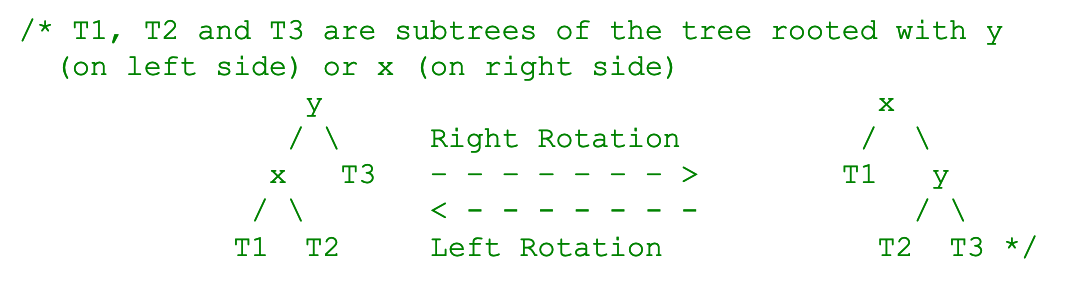
\includegraphics[width=\linewidth]{treap_heap_property.png}
    \end{center}

    \begin{solution}
    \lstinputlisting[language = python]{treap_solution_1.py}
    \end{solution}
    \begin{solution}
        \lstinputlisting[language = python]{treap_solution_2.py}
    \end{solution}
    
\end{Exercice}



\end{document}